\section{Unified RSI Experiment Organization}
\label{sec:organization}

\fwname separates RSI methods from evaluation benchmarks to accommodate differences in implementation, task inputs, and scoring. This section describes how methods are packaged as skills and how agents organize the experiment automatically.

\begin{table*}[t]
  \centering
  \small
  \caption{The nine built-in modular RSI methods in \fwname.}
  \label{tab:methods}
  \begin{tabular}{@{}p{.10\textwidth}p{.17\textwidth}p{.37\textwidth}p{.25\textwidth}@{}}
    \toprule
    \textbf{Method} & \textbf{Category} & \textbf{Self-improvement mechanism} & \textbf{Updated artifact} \\
    \midrule
    Default & Reflection loop & Evaluate, diagnose failures in traces, edit the state, and validate snapshots. & Agent instructions and domain skills \\
    APE & Discrete prompt optimization & Propose candidate instructions from task examples and retain the best after evaluation. & Selected task instructions \\
    OPRO & Discrete prompt optimization & Condition the optimizer on past instructions and scores to propose new instructions. & Improved task instructions and score history \\
    ACE & Workflow and experience evolution & Reflect on training traces and incrementally curate a structured playbook. & Structured playbook \\
    AWM & Workflow and experience evolution & Distill reusable routines from successful traces and freeze them for held-out testing. & Reusable workflow memory \\
    OpenSkill & Modular skill evolution & Retrieve domain knowledge and refine a reusable skill library through virtual trials. & Refined domain skill library \\
    SkillAdam & Modular skill evolution & Use trace feedback, a dynamic issue tracker, and a budgeted paired evaluation to evolve skills. & Evolved skills and issue history \\
    SkillOpt & Modular skill evolution & Use bounded edits, candidate evaluation, and reflection across rounds. & Locally revised skill modules \\
    TRACE & Contrastive trace and skill evolution & Learn from contrasting traces during continuous containerized training and test the best training checkpoint. & Skill checkpoint derived from contrasting traces \\
    \bottomrule
  \end{tabular}
\end{table*}


\subsection{Modular RSI Skills}

An RSI method often comes with a custom training loop that parses tasks, assembles meta-prompts, and updates the agent configuration. In \fwname, each method is represented as a structured skill. The \emph{Super Agent}, which coordinates the experiment, loads the selected skill on demand and follows its procedure.

\paragraph{Controlled state updates.}
Each skill modifies the prompts or skill library of the same \emph{Target Agent} through a common file interface. The default method can edit the main instruction file and the skill library. OPRO, APE, ACE, and AWM create a dedicated skill file for optimized instructions, rules, or workflow memory and add a fixed reference in the main instruction file. The update loop then edits the dedicated file. SkillAdam, SkillOpt, OpenSkill, and TRACE directly synthesize, prune, and reorganize domain skills in the Target Agent's skill directory. Table~\ref{tab:methods} summarizes the nine built-in methods. The researcher can switch methods on the same benchmark by selecting a different RSI skill.

\subsection{Agent-Orchestrated Automated RSI and Evaluation}
\label{sec:orchestration}

After the user selects a Target Agent, an RSI skill, and a benchmark, the Super Agent coordinates initialization, training, and held-out testing (Figure~\ref{fig:rsi-workflow}). It loads the selected RSI skill and takes a snapshot of the Target Agent's initial file state \(S_0\). Training then proceeds in rounds over the training split.

\begin{figure*}[t]
  \centering
  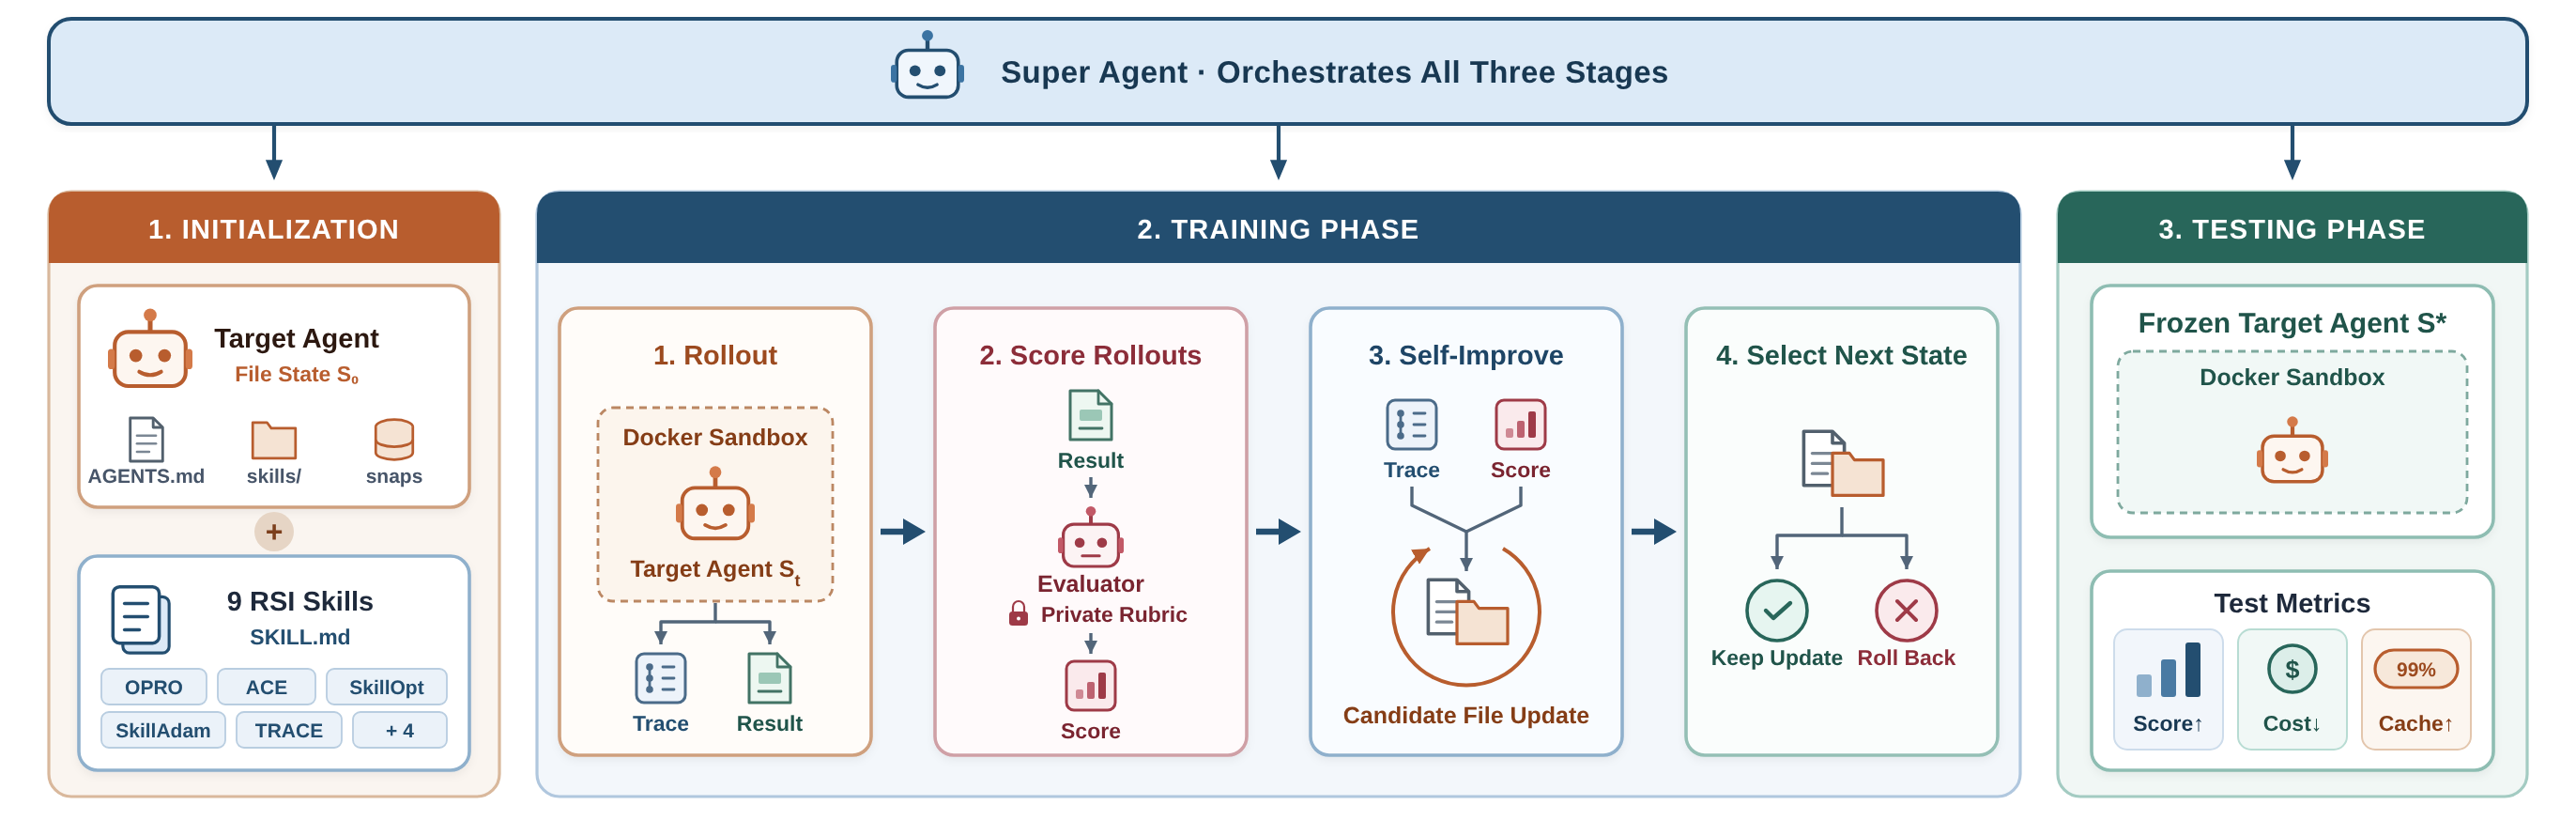
\includegraphics[width=\textwidth]{figs/fig1-preview.png}
  \caption{The unified RSI workflow in \fwname. The Super Agent coordinates initialization, training, and held-out testing. The Target Agent runs tasks in Docker and produces a trace and a task result. The Evaluator scores the task result using a private rubric. The selected RSI method uses the trace and score to propose changes to the Target Agent's files. Its selection rule keeps the update or restores the previous state. Held-out tests use the frozen state.}
  \label{fig:rsi-workflow}
\end{figure*}

\begin{enumerate}
  \item \textbf{Rollout.} The Target Agent receives a public task statement, executes the task in an isolated container, and produces an execution trace and a task result.
  \item \textbf{Scoring.} An Evaluator subagent scores the task result under a private rubric and returns a structured evaluation record to the Super Agent.
  \item \textbf{Self-improvement.} The selected RSI method uses the execution trace and evaluation score to propose changes to the Target Agent's instructions or skill library. The method specifies which training role produces the update.
  \item \textbf{State selection.} The RSI method applies its selection rule to keep the proposed file update or restore the previous state.
\end{enumerate}

When training ends, the Super Agent freezes the selected state \(S^*\) as read-only, dispatches runs on the held-out split, and aggregates the final metrics.

\paragraph{Containerized benchmarks and isolated evaluation.}
\fwname provides seventeen containerized benchmarks drawn from multiple domains. Each case separates the public task statement from private scoring criteria. To keep private scoring material out of the update loop, the experiment uses the subagent delegation primitive to dispatch an Evaluator, which runs the Target Agent in an isolated environment and scores its execution. The Evaluator's structured response contains a numeric score, duration, cost, and a session identifier. The identifier links the score to its execution trace for diagnosis, while the scoring criteria stay with the Evaluator.
